\documentclass{article}
\usepackage[utf8]{inputenc}
\usepackage[T1]{fontenc}
\usepackage{xcolor}
\usepackage{hyperref}
\usepackage{bookmark}
\usepackage{amsthm}
\usepackage[most,skins]{tcolorbox}
\usetikzlibrary{positioning,calc}
\usepackage{fontawesome5}
\usepackage[a4paper, margin=1in]{geometry}
\usepackage{fancyhdr}
\usepackage{listings}
\usepackage{fancyvrb}


\title{Free Website Guide}
\author{}
\date{\today}
\hypersetup{
    colorlinks=true,
    linkcolor=blue,
    filecolor=magenta,
    urlcolor=blue,
    pdftitle={Free Website Guide},
    pdfpagemode=FullScreen,
}

% listings setup for code snippets

\definecolor{codebg}{rgb}{0.97,0.97,0.97}
\definecolor{codeframe}{rgb}{0.2,0.2,0.7}

\lstset{
  language=HTML,
  basicstyle=\ttfamily\small,
  backgroundcolor=\color{codebg},
  frame=lines,
  framexleftmargin=5pt,
  framextopmargin=2pt,
  framexbottommargin=2pt,
  rulecolor=\color{codeframe},
  breaklines=true,
  breakatwhitespace=true,
  captionpos=b,
  tabsize=2,
  numbers=none,
  showstringspaces=false,
  extendedchars=true,
  escapeinside={\(*}{*\)},
  fancyvrb=true,
  firstnumber=1,
  xleftmargin=15pt,
  frame=tb,
  framerule=1pt,
  belowcaptionskip=10pt,
  abovecaptionskip=10pt,
  breakautoindent=true,
  breakindent=0pt,
  morecomment=[l]{//},
  keywordstyle=\color{blue},
  commentstyle=\color{gray},
  stringstyle=\color{red},
title=\lstname}
\lstdefinestyle{withbreaks}{
  breaklines=true,
  breakatwhitespace=true,
  frame=lines,
  framesep=5pt,
  rulesepcolor=\color{codeframe},
  framexleftmargin=5pt,
  framextopmargin=5pt,
  framexbottommargin=5pt
}


% Set up the document layout

\setlength{\parindent}{0pt}
\setlength{\parskip}{1em}
\setlength{\textwidth}{15cm}
\setlength{\oddsidemargin}{0cm}
\setlength{\evensidemargin}{0cm}
\setlength{\topmargin}{-1cm}
\setlength{\textheight}{23cm}
\setlength{\headheight}{0cm}
\setlength{\headsep}{0cm}
\setlength{\footskip}{1cm}
\setlength{\marginparwidth}{0cm}
\setlength{\marginparsep}{0cm}
\setlength{\columnsep}{1cm}
\setlength{\parskip}{1em plus 0.5em minus 0.5em}
\setlength{\parindent}{0pt}

% Definition Box
\newtcolorbox{definition}[1]{%
  colback=blue!5!white,
  colframe=blue!80!black,
  fonttitle=\sffamily\bfseries\large,
  fontupper=\sffamily,
  title=Definition: {\usefont{T1}{pzc}{m}{it}#1},
  boxrule=1pt,
  arc=4pt,
  left=3mm,
  right=3mm,
  top=2mm,
  bottom=2mm,
  enhanced,
  sharp corners=south,
  drop shadow,
  before skip=10pt,
  after skip=10pt,
  halign=justify,
  valign=center
}

% Concept Box
\newtcolorbox{concept}[1]{%
  colback=green!5!white,
  colframe=green!80!black,
  fonttitle=\sffamily\bfseries\large,
  fontupper=\sffamily,
  title=Concept: {\usefont{T1}{pzc}{m}{it}#1},
  boxrule=1pt,
  arc=4pt,
  left=3mm,
  right=3mm,
  top=2mm,
  bottom=2mm,
  enhanced,
  sharp corners=south,
  drop shadow,
  before skip=10pt,
  after skip=10pt,
  halign=justify,
  valign=center
}


\begin{document}

\maketitle

\tableofcontents
\newpage

% Main contents
\section{Preface}

This document will walk you through the process of creating a free, publicly accessible website. The guidance provided is intended to be straightforward and accessible, ensuring that even those with minimal technical expertise can follow along. Anyone with a basic understanding of how to use a computer and navigate the internet should be able to follow the instructions without too much difficulty. Readers may range from absolute beginners—those who have never written a single line of HTML—to experienced programmers who wish to streamline their workflow by leveraging free resources.
\subsection{Introduction}
This document serves as a comprehensive guide for anyone interested in creating a free website. It covers the essential steps and considerations involved in setting up a website without incurring any costs. The focus is on providing clear, step-by-step instructions that are easy to follow, regardless of the reader's prior experience with web development or hosting.
\subsection{Purpose of this Document}

This document aims to empower readers with the knowledge and tools necessary to establish an online presence without any initial financial investment. It will cover the fundamental aspects of web hosting, domain registration, and website creation, ensuring that readers can successfully launch their own websites using free resources available online.

\subsection{Target Audience}

This document is intended for a broad audience of individuals who wish to create a website without a budget for premium development tools or hosting. Specifically, it is suitable for:

\begin{itemize}
    \item Students and educators who require a platform to showcase projects, portfolios, or learning materials.
    \item Hobbyists and content creators aiming to share writing, art, photography, or other personal work online.
    \item Small organizations, clubs, and community groups looking to establish a web presence.
    \item Aspiring developers who wish to gain practical experience with web development tools and workflows.
    \item Freelancers and independent professionals who seek to demonstrate services through a self-built website.
\end{itemize}

\subsection{Scope of the Document}

The scope of this document encompasses all phases of free website creation, placing primary emphasis on development tasks. It includes:

\begin{itemize}
    \item \textbf{Planning and Requirements Gathering:} Defining purpose, target audience, content inventory, and user experience goals.
    \item \textbf{Technology Selection:} Comparing static site generators (e.g., Jekyll, Hugo), lightweight JavaScript frameworks (e.g., Vue, Svelte), or pure HTML/CSS approaches.
    \item \textbf{Development Environment Setup:} Installing and configuring free code editors (e.g., Visual Studio Code), package managers (e.g., npm), and version control systems (e.g., Git).
    \item \textbf{Design and Layout:} Crafting responsive page layouts using free CSS frameworks (e.g., Tailwind CSS, Bootstrap) or custom CSS methodologies (e.g., Flexbox, Grid).
    \item \textbf{Writing Code:} Authoring HTML templates, modular CSS, and JavaScript for interactive elements; structuring files and directories for scalability.
    \item \textbf{Content Management:} Incorporating markdown or other plain-text formats to author content, enabling straightforward updates without proprietary software.
    \item \textbf{Asset Optimization:} Compressing images, minifying scripts and styles, and lazy-loading resources to ensure rapid page load times on free hosting.
    \item \textbf{Testing and Debugging:} Utilizing free browser development tools (e.g., Chrome DevTools, Firefox Developer Edition) and open-source testing frameworks (e.g., Lighthouse, ESLint).
    \item \textbf{Deployment Overview:} Brief discussion of free deployment platforms (e.g., GitHub Pages, Netlify, Vercel), Continuous Integration/Continuous Deployment (CI/CD) pipelines, and basic DNS configuration for free custom domain services.
    \item \textbf{Maintenance and Updates:} Strategies for version control, content updates, security patches, and performance monitoring using free analytics tools.
    \item \textbf{Transition to Paid Services (Optional):} Guidelines for when and how to upgrade to a paid service for domain name registration, premium hosting, or advanced features, including:
    \begin{itemize}
        \item Criteria for upgrading based on traffic, functionality requirements, or security concerns.
        \item Comparison of paid hosting providers and domain registrars.
        \item Migration steps from free to paid environments, ensuring minimal downtime.
    \end{itemize}
\end{itemize}

\subsection{Document Structure}

The document is structured to guide readers through the process of creating a free website, starting from the initial planning phase to the final deployment and maintenance. Each section builds upon the previous one, ensuring a logical flow of information. Terms and concepts are introduced progressively, with practical examples and exercises to reinforce learning. The document also includes references to additional resources for readers who wish to explore specific topics in greater depth.

\subsection{Assumptions and Prerequisites}

This document assumes that readers have basic computer literacy, including the ability to navigate the internet, install software, use a web browser, and manage files on their local machine. Familiarity with basic programming concepts is helpful but not required. The document will introduce necessary technical terms and concepts as they arise, ensuring that all readers can follow along regardless of their prior knowledge.
\section{Setting up files and services}

The first step in creating a free website is to set up the necessary files and services. This section will guide you through the process of preparing your development environment, selecting a hosting service, and organizing your project files.

\subsection{Choosing a Hosting Service}

\subsubsection{What is a Hosting Service?}
A hosting service is a company that provides the infrastructure and technology needed to make your website accessible on the internet. They store your website's files on their servers and ensure that they are available to users who visit your site. Hosting services can vary widely in terms of features, performance, and cost. It is possible to host a website yourself, but for most users, especially those new to web development, using a hosting service is the most practical option. There are several free hosting services available that allow you to host your website without any cost. Some popular options include:
\begin{itemize}
    \item \textbf{GitHub Pages:} Ideal for simple websites, it allows you to host your site directly from a GitHub repository.
    \item \textbf{Netlify:} Offers free hosting with continuous deployment from Git repositories, making it easy to update your site.
    \item \textbf{Vercel:} Similar to Netlify, it provides free hosting with a focus on performance and ease of use.
    \item \textbf{Firebase Hosting:} Great for dynamic web applications, it offers free hosting with a generous quota.
    \item \textbf{Surge:} A simple command-line tool for publishing static sites, ideal for quick deployments.
\end{itemize}

For this guide, we will focus on using GitHub Pages as it is widely used and integrates well with version control. However, the principles outlined here can be applied to any of the mentioned services. Make sure to sign up for an account with your chosen hosting service before proceeding.

\subsubsection{GitHub Pages}
GitHub Pages is a free hosting service provided by GitHub that allows you to host websites directly from a GitHub repository. It is designed to work seamlessly with Git, making it easy to deploy your site by simply pushing changes to your repository. GitHub Pages is an excellent choice for personal projects, portfolios, and documentation sites, as it supports custom domains and out-of-the-box HTTPS. It is well suited for developers, as it allows you to leverage Git's version control capabilities while providing a straightforward way to publish your work online.

\paragraph{Creating a GitHub Account}
To get started with GitHub Pages, you'll need a GitHub account. If you don't have one already, follow these steps to create an account:
\begin{enumerate}
    \item Go to the \href{https://github.com/}{GitHub website}.
    \item Click on the ``Sign up'' button in the upper right corner.
    \item Fill out the registration form with your details and click ``Create account''.
    \item Verify your email address by clicking the link sent to your inbox.
    \item Once your account is created, you can log in to GitHub.
\end{enumerate}

\paragraph{Creating a Repository}
A repository is where your website's files will be stored on GitHub. To create a new repository for your website, follow these steps:
\begin{enumerate}
    \item Log in to your GitHub account \href{https://github.com/login}{here}.
    \item Click on the ``+'' icon in the upper right corner and select ``New repository''.
    \item Enter a name for your repository (e.g., ``my-website'') and add a description if desired.
    \item Leave the repository as ``Public'' as it is required for GitHub Pages to work for free hosting.
    \item Everything else can be left as default, but you can choose to initialize the repository with a README file if you wish.
    \item Click the ``Create repository'' button to finish.
\end{enumerate}

\subsection{Setting Up Your Local Development Environment}

Before you can start building your website, you'll need to set up your local development environment. This involves installing the necessary software and tools that will allow you to create and manage your website files effectively.

\subsubsection{Installing Git}
Git is a version control system that allows you to track changes in your code and collaborate with others. It is essential for managing your website's source code, especially when using GitHub Pages. To install Git, follow these steps:
\begin{enumerate}
    \item Go to the \href{https://git-scm.com/downloads}{Git website}.
    \item Download the appropriate version for your operating system (Windows, macOS, or Linux).
    \item Follow the installation instructions for your platform. During installation, you can choose the default options unless you have specific preferences.
    \item Once installed, open a terminal or command prompt and verify the installation by typing \texttt{git --version}. You should see the installed version of Git displayed.
\end{enumerate}

\subsubsection{Installing a Code Editor}
A code editor is a software application that allows you to write and edit your website's code. For this guide, we recommend using Visual Studio Code (VS Code) due to its popularity and extensive features. To install VS Code, follow these steps:
\begin{enumerate}
    \item Go to \href{https://code.visualstudio.com/}{Visual Studio Code website}.
    \item Download the version for your operating system (Windows, macOS, or Linux).
    \item Follow the installation instructions for your platform.
    \item Once installed, open VS Code and familiarize yourself with its interface. You can customize the settings and install extensions to enhance your coding experience.
\end{enumerate}

\subsubsection{Creating Your Project Files}
Now that you have Git and a code editor installed, you can create the initial files for your website project. Follow these steps to set up your project structure:
\begin{enumerate}
    \item Create a new folder on your local machine where you want to store your development files (e.g., \texttt{DEV}).
    \item Inside the \texttt{DEV} folder, right-click and open VS Code. This will open the folder in the editor, allowing you to create and manage your project files easily.
    \item Press \texttt{Ctrl~+~Shift~+~\`} (or \texttt{Cmd~+~Shift~+~\`} on macOS) to open a new terminal window within VS Code.% chktex 14
    \item Go to your remote repository on GitHub and copy the repository URL (e.g., \texttt{https://github.com/your-username/my-website.git}).
    \item In the terminal, enter the following command to clone your GitHub repository:
    \begin{verbatim}
        git clone <repository-url>
    \end{verbatim}
    Replace \texttt{<repository-url>} with the URL you copied earlier. This will create a local copy of your repository in the \texttt{DEV} folder.
    \item Click File~$\rightarrow$~Open Folder in VS Code and select the folder you just cloned. This will open your project in the editor.
\end{enumerate}



\newpage
\section{How Static Websites Work}

\subsection{Definitions and Concepts}
\begin{definition}{Static Website}
A static website is a type of website that delivers the same content to every user. It is built using HTML, CSS, and JavaScript, and the files are served directly to the user's browser without any server-side processing. Static websites are typically faster and more secure than dynamic websites, as they do not rely on databases or server-side scripts.
\end{definition}

\begin{definition}{HTML}
HTML (HyperText Markup Language) is the standard markup \\ language used to create the structure and content of web pages. It defines elements such as headings, paragraphs, links, images, and other multimedia content. HTML files are static and do not change unless manually edited.% \\ is to make sure the text is not too long
\end{definition}

\begin{definition}{CSS}
CSS (Cascading Style Sheets) is a stylesheet language used to describe the presentation of HTML documents. It allows you to control the layout, colors, fonts, and overall appearance of your website. CSS files are also static and are linked to HTML files to apply styles.
\end{definition}

\begin{definition}{JavaScript}
JavaScript is a programming language that enables interactive features on web pages. It can manipulate HTML and CSS, respond to user actions, and perform calculations. While JavaScript can be used in static websites, it is often associated with dynamic websites where server-side processing is involved.
\end{definition}

\begin{concept}{Local Development Versus Live Website}
When developing a static website, you typically work on your local machine using a code editor. This allows you to create and test your website files before deploying them to a live server. Once you are satisfied with your local version, you can upload the files to a hosting service, making them accessible to users on the internet.
\end{concept}

\subsection{How Static Websites Work}
Static websites work by serving pre-built HTML, CSS, and JavaScript files directly to the user's browser. When a user requests a static web page, the server retrieves the corresponding HTML file and sends it to the browser.\\ The browser then interprets the HTML, applies any linked CSS styles, and executes any JavaScript code to render the page. This process is straightforward and does not require any server-side processing, making static websites fast and efficient.

\vspace*{1cm}

\noindent\hspace*{0cm}
\begin{tikzpicture}[
    node distance=3cm and 3cm,
    every node/.style={font=\small\sf, align=center},
    box/.style={draw=blue!50!black, fill=blue!10, thick, rounded corners, minimum width=3.2cm, minimum height=1.2cm},
    filebox/.style={draw=orange!60!black, fill=orange!10, thick, rounded corners, minimum width=3.2cm, minimum height=1.2cm},
    arrow/.style={->, very thick, >=stealth}
]

% Nodes
\node[box] (user) {User\\(Web Browser)};
\node[box, right=of user] (internet) {Internet};
\node[box, right=of internet] (server) {Web Server\\(Hosting Provider)};
\node[filebox, below=of server] (files) {Static Files:\\HTML, CSS, JS};

% Arrows
\draw[arrow] 
  ([yshift=5pt]user.east) -- node[above, yshift=2pt]{1. Request Page} 
  ([yshift=5pt]internet.west);

\draw[arrow] 
  ([yshift=-5pt]internet.west) -- node[below, yshift=-2pt]{5. Deliver Page} 
  ([yshift=-5pt]user.east);

\draw[arrow] (internet) -- node[above]{2. Forward Request} (server);
\draw[arrow] (server) -- node[right]{3. Fetch Files} (files);

\draw[arrow] 
  (files.west) 
  to[out=180, in=-90] 
  node[midway, below left, font=\small\sf] {4. Send Files}
  ($(internet.south)+(0,-1.5)$) 
  to[out=90, in=270] 
  (internet.south);

\end{tikzpicture}

\vspace*{1cm}

This diagram illustrates the flow of a static website request:
\begin{enumerate}
    \item The user opens a web browser and requests a specific page by entering a URL.\ 
    \item The request is sent over the internet to the web server hosting the static files.
    \item The server retrieves the requested HTML file along with any associated CSS and JavaScript files.
    \item The server sends these files back to the user's browser.
    \item The browser renders the page, applying styles and executing scripts as needed.
\end{enumerate}



\end{document}
